\documentclass{standalone}
\usepackage{tikz}
\usepackage{ctex,siunitx}
\usepackage{tkz-euclide}
\usepackage{amsmath}
\usetikzlibrary{patterns, calc}
\usetikzlibrary {decorations.pathmorphing, decorations.pathreplacing, decorations.shapes,}
\begin{document}
\small
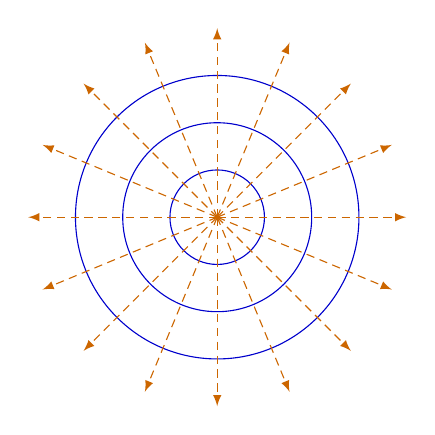
\begin{tikzpicture}[>=latex,scale=0.6]
  \foreach \x in {1,2,3}
  {
    \draw[blue!80!black] (0,0) circle (\x);
  }
  \foreach \x in {0, 22.5, 45, ..., 337.5}
  {
    \draw[->, densely dashed, orange!80!black](0,0)--(\x:4);
  }   
\end{tikzpicture}
\end{document}